\chapter{AsthmAPP}
\label{chp:description}

This chapter gives a description of AsthmAPP, through textual description and screenshots. Note that the main language of the application is Norwegian. We have translated the text where it seemed appropriate. 

\section{Architecture and Technology}

\subsection{System Architecture}
\label{sec:architecture}
Figure \ref{fig:basic-architecture} shows an overview of the architecture we used for our products (\ab{} included). We reused some of the components Aaberg et. al. created during Customer Driven Project\cite{CustomerDriven}. 

Data is stored at a MySQL database hosted by NTNU. \app{} and \ab{} access the database through a webservice written in PHP, which is also hosted by NTNU. The reason for accessing the database through a webservice is twofold. First, it is difficult to access the database when a device is not located on the local network at NTNU. It would be required that a user has configured VPN\footnote{Virtual Private Network} in order to access the NTNU network. We also can not assume that users have access to the network at NTNU.

Secondly, by having a webservice that structures the results given by the database, it becomes easier for the client to deserialize these results, as they are served as JSON-objects\footnote{JavaScript Object Notation}.    

When one of the applications wants to store data to the database, it does a HTTP POST, with the data as POST parameters, to a predefined route on the webservice. When the application wants to retrieve data from the database, it does a HTTP GET to the webservice, which extracts the data requested from the database, formats it to JSON, and returns the data to the application.  

By having a webservice layer between the applications and the database, the system scalability suffers, but modifiability is increased, which we considered as a good trade-off at the current state of our project. 

\begin{figure}
		\centering
			\fbox{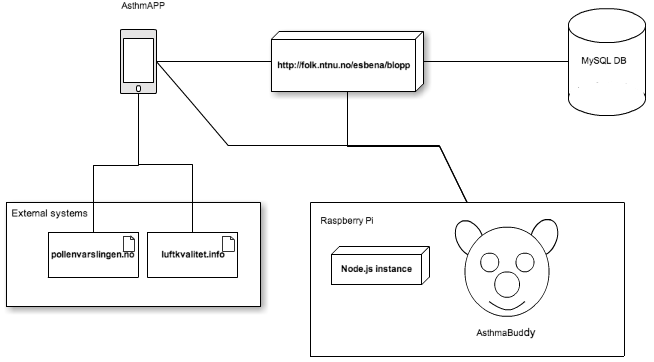
\includegraphics[width=0.60\paperwidth]{Pictures/system-architecture.png}}
		\caption{System Architecture}
		\label{fig:basic-architecture}
\end{figure}

\clearpage{}

\subsection{Technology and Frameworks Used in AsthmAPP}
\label{sec:techandframeinapp}
\app{} is developed in native Android code, which implies using Java as the programming language and the Android Application Framework\fnurl{Android Application Framework}{http://developer.android.com/develop/index.html}. Additionally, we used the following frameworks to ease the development: 


\textbf{Gson} 

As mentioned in previously, our webservice gives out JSON-formatted objects of data stored in our database. We used Google's Gson-library\fnurl{Google Gson}{https://code.google.com/p/google-gson/} to deserialize JSON objects into Java objects.

\textbf{JodaTime} 

Java's default implementation of time is cumbersome to work with, with a lot of it's functionality deprecated. JodaTime\fnurl{JodaTime}{http://www.joda.org/joda-time/} is an open source project that seeks to handle time in a proper manner on the Java platform\footnote{Oracle has promised that Java 8 has better support for managing time, but Java 8 was released at a time at which our program was already operative.}.


\section{Design Rationale}
\label{sec:usability-affect-design}
While designing AsthmAPP, we strived for an easy-to-use design with a good overview, in addition to the Android Design Principles\cite{androiddesign}. We have also taken Shneidermann's eight golden rules into consideration when designing \app{}\cite{shneiderman2003designing}. 
We tried to lighten the short-term memory load by using a combination of sounds, pictures and text to tell the user the options that are available or what is expected from the user. 

The application is divided into two partitions, one for the parents and one for the children. In order to access one of the partitions, the user clicks on one of the buttons shown in Figure \ref{fig:asthmapp-main-menu}. The main menu of both partitions of \app{} gives a general overview. \app{} does not provide shortcuts between different modules, e.g. a parent who is currently viewing the medicine log has to go back to the main menu in order to view the treatment plan. While this breaks with Shneidermann's rules and the Android design principles, we believed that the solution we found was the preferrable one.  

During a treatment the child is prompted to take action in order to continue through the process, giving the child a locus of control. 

\section{Use of Gamification in \app{}}
\label{sec:useofgamificationinapp}

\subsection{Design Rationale for Gamification System in \app{}}
\label{sec:designrationalegamification}
In AsthmAPP we aimed to use gamification as a distraction and rewarding element for the children. During the start of the project we arranged a brain-storming session to find which gamification techniques we wished to add to \app{} and \ab{}. The summary of this session is listed in Section \ref{sec:combininggamemechanismsinasthmapp}. 

At first thought, we figured that implementing an avatar system was a smart approach to create a gamification system. An avatar system gives possibilities for expansion in order for the application to combat boredom in the long run. When developing avatar systems, a key for its success is that it is balanced and good looking. After having spent a few hours programming an avatar system, we chose to discard the functionality, caused by the lack of skills necessary to make it attractive. 

We chose to aim for a system we were sure we were able to implement in a well-working fashion in order to test the system with users. We expanded on Aaberg \etal{}'s use of experience points (represented by stars), by adding a shop where the stars may be used for purchasing rewards. We believed this system has many possibilites for expanding upon on a later stage. The parents have the possibility to create their personalized gamification environment through the reward system. This solution stands to reason with the arguments of Nicholson regarding how to design gamification\cite{nicholson2012user}.

The children are rewarded with stars based on their health state. The rationale behind this is that the children may have to take more medicine when they have a cold or there is a lot of pollen in the air. The parents have access to a administrator menu where they may add new rewards for the children. The children will then be able to order the rewards when they have earned a sufficient number of stars. This way the parents and their children create their own gamification environment. Examples of possible rewards could be to give the child an extra 10 NOK in weekly allowance, taking him/her to soccer matches or even to the local amusement park. It is an option where the only boundary is the imagination and how much cost and effort parents wish to invest in it.    

The rewards will appear on a ``milestone'' basis. We do not want children to feel that they lose something if they spend stars on a reward. We do not want to force parents into giving away rewards they can not afford or do not wish to give. The use of the reward system is optional and decided by the user, making the user in control of how they wish to gamify the experience. 
We do not wish to have the children spending too much time using the application, since using a tablet or phone at such a young age is considered unhealthy. This had some implications on the complexity of our gamification system. 


\subsection{Gamification Elements in AsthmAPP}
\label{sec:combininggamemechanismsinasthmapp}

\begin{onehalfspacing}
\begin{table}[H]
\begin{tabular}{| p{2.5cm} | p{2.1cm} | p{9.5cm} | }
	\hline
	\textbf{Mechanism} & \textbf{Included in AsthmAPP} & \textbf{Rationale} \\
	\hline
	Avatar systems & No & We did not have time to implement this during our thesis, but we do believe this could be a good feature if it was implemented in a right manner.    
	 \\
	\hline
	Achievements and badges & No & We believe our target group will not enjoy this feature as much as older children, e.g. those of 12 - 16 years of age.  \\
	\hline 
	Real-World rewards & Yes & Children enjoy the feeling of being rewarded with something real.
	 \\
	\hline
	Mirroring user behavior & Yes & Demonstration has a positive effect on children.
	\\
	\hline
	Leaderboards & No & There are no way to implement this in a realistic and legal way. Children would have to share their data, which consists of points based on medicine doses. Parents could be blamed if their child were on the bottom of the list. It would also be negative for small children's motivation if their effort is not reflected on the leaderboard. 
	\\
	\hline
	Social networking & No & Much of the same reasons as why we did not choose leaderboards. We also believe that children in our target group would not understand this aspect.  
	\\
	\hline
	Progress bar & No & In an ideal world, we could have shown how close the child was to becoming fully treated for asthma. However, identifying how close a patient is to becoming healthy, is virtually impossible. Another usage may be to match the child's progress for each week against his/her medicine plan. This would however, imply that by-need treatments would not be included, which may seem unfair for the child. Additionally, their progress would be deleted every week, which would not have much motivational effect.  
	\\
	\hline
	Experience points & Yes & The stars will work as experience points, which may used to cash in rewards from the parents. 
	\\
	\hline
	Contests & No & Using medical history to participate in contests would be a violation of Norwegian privacy laws. It may also be used to pinpoint ``bad'' parents.      
	\\
	\hline
\end{tabular}
\caption{Assessment of different game mechanisms}
\label{tab:game-mech-in-astmapp}
\end{table}
\end{onehalfspacing}


\clearpage{}

\section{Child partition}
\label{sec:description-child-partition}

A screenshot of the first view users meet is included in Figure \ref{fig:asthmapp-main-menu}. By pressing the top button, the user is brought to the child partition of \app{}. 

\begin{figure}[H]
	\centering
	\fbox{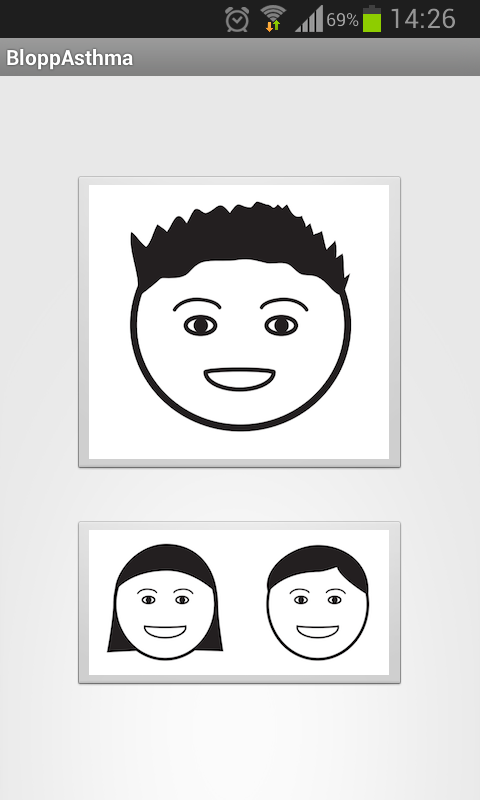
\includegraphics[width=0.25\paperwidth]{Pictures/app-screenshots/asthmapp-main-menu.png}}
	\caption{Start menu of \app{}.}
	\label{fig:asthmapp-main-menu}
\end{figure}

The child partition of our application consists of four parts. This parts are the treatment process, the treasure chest, the reward shop and the instructions for how to finish a treatment.

\subsection{Treatment}
\label{sec:sec:description-treatment}
Figure \ref{fig:capp_start_treatment} shows a screenshot for the application when the child starts his/her treatment. This sequence may be started by on of two events: (i) \emph{The child reacts to an alarm set in the parent partition}, or (ii) \emph{The child needs to take his/her medicine by need}. If (ii) is the case, the child is instructed to pick the medicine from a list shown by the application. If (i) is the case, the medicine is determined beforehand. When a child has started his/her treatment, he/she is taken through an animated sequence, which reacts when a child interacts with the device. The child is being told what to do by the comforting voice of Andreas Ystmark\footnote{A classmate of ours at NTNU}.  


\subsection{Showing Collected Stars}
\label{sec:description-show-rewards}
Figure \ref{fig:capp_stars} shows a screenshot for the application when the child wants to review how many stars he/she has received, based on the amount of treatments completed. Since we cannot assume that the child is able to read, we have made the stars countable, and hopefully the child is able to comprehend how many stars he/she actually has. We also provide some help to those who are able to read numbers, by showing the number of stars a child has on the top of the screen.      

\subsection{Shop}
\label{sec:description-shop}
In the shop, children are allowed to select rewards given by their parent(s). Figure \ref{fig:child-possible-rewards} and \ref{fig:child-bought-rewards} show an inside-view of our shop. Children can buy a reward by pressing the selected reward in the menu. Due to time constraints and lack of good software solutions, we have not been able to implement a voice over, so the children may need help with reading the names of the rewards. The possibility of adding pictures to represent the reward should make it easier for the children. 


\subsection{Treatment Instructions}
\label{sec:description-instructions}
The treatment instructions is a book-styled instruction set which shows generically how to take the medicine. 
The following steps are included in the instructions: 
\begin{enumerate}
  \item Shake the inhaler to loosen the particles. 
  \item Take the cap of the inhaler.
  \item Attach the inhaler to the inhaling chamber.
  \item Cover nose and mouth with the inhaling chamber.
  \item Press the inhaler until you hear a sound.
  \item Let the child breathe calmly in and out 10 times.
  \item Let the child wash his/her mouth.
\end{enumerate} 

\begin{figure}
	\begin{minipage}[t]{0.3\linewidth}
		\centering
			\fbox{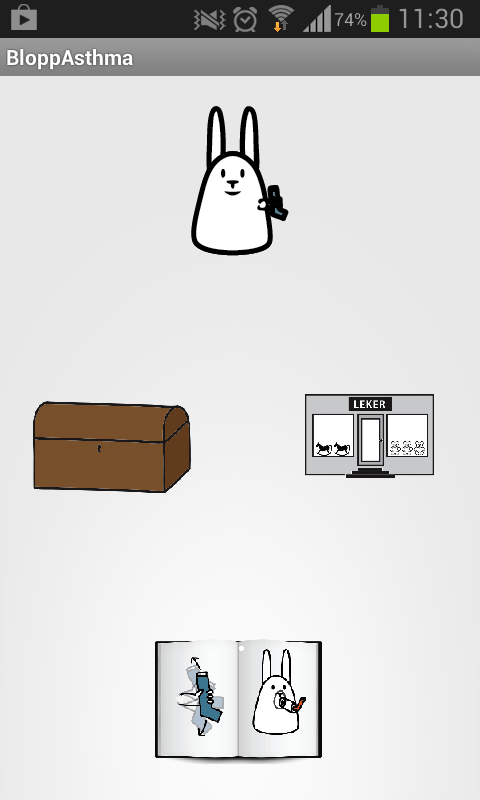
\includegraphics[width=0.20\paperwidth]{Pictures/new-screenshots/kid-menu.png}}
		\caption{Main menu of child \\ partition}
		\label{fig:child-menu}
	\end{minipage}
	\hspace{0.5cm}
	\begin{minipage}[t]{0.3\linewidth}
		\centering
			\fbox{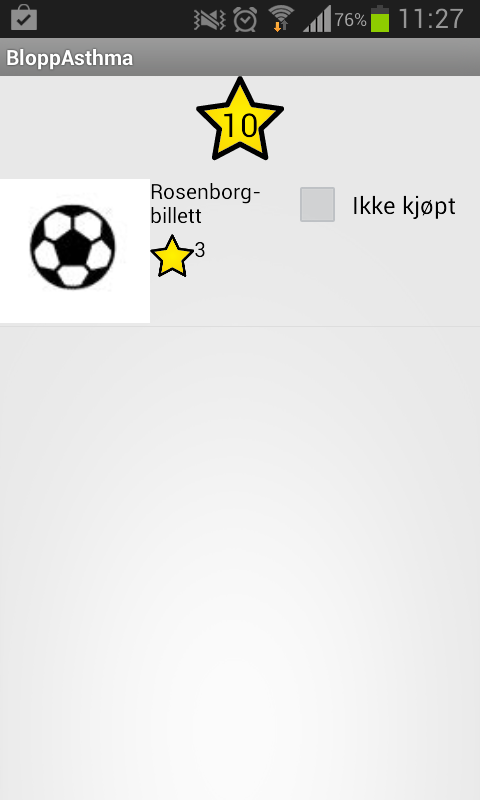
\includegraphics[width=0.20\paperwidth]{Pictures/new-screenshots/child-possible-rewards.png}}
		\caption{\\ Possible rewards a child can choose from}
		\label{fig:child-possible-rewards}
	\end{minipage}
	\hspace{0.5cm}
	\begin{minipage}[t]{0.3\linewidth}
		\centering
			\fbox{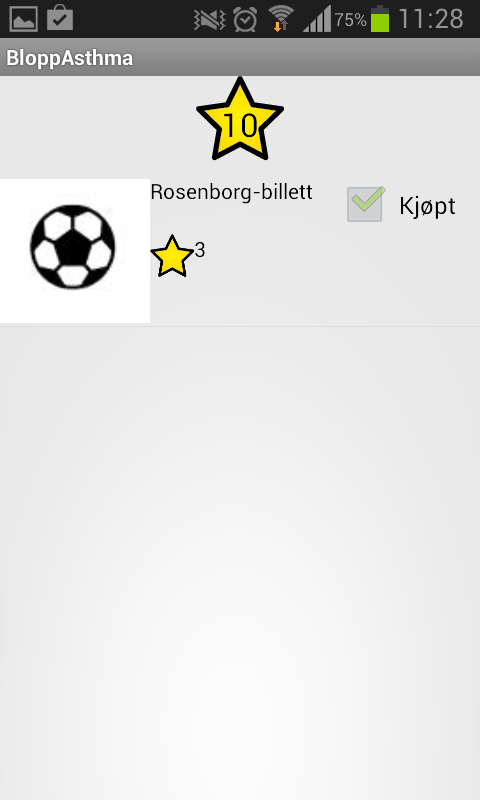
\includegraphics[width=0.20\paperwidth]{Pictures/new-screenshots/child-bought-reward.png}}
		\caption{A child has bought the reward}
		\label{fig:child-bought-rewards}
	\end{minipage}
\end{figure}

\begin{figure}
	\begin{minipage}[t]{0.4\linewidth}
		\centering
			\fbox{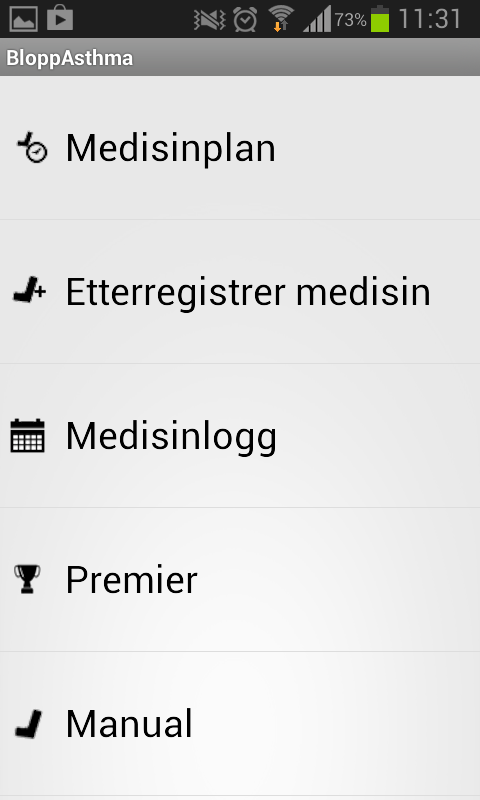
\includegraphics[width=0.20\paperwidth]{Pictures/new-screenshots/parent-menu.png}}
		\caption{Main menu of partent partition}
		\label{fig:parent_main_menu}
	\end{minipage}
	\hspace{3cm}
	\begin{minipage}[t]{0.4\linewidth}
		\centering
			\fbox{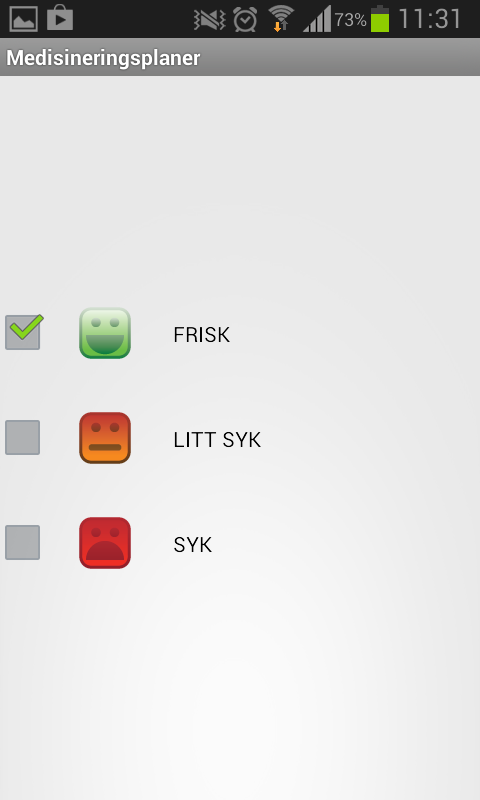
\includegraphics[width=0.20\paperwidth]{Pictures/new-screenshots/medicine-plans.png}}
		\caption{Available medicine plans}
		\label{fig:parent_medicine_plans}
	\end{minipage}
	%NEW LINE
	\begin{minipage}[t]{0.4\linewidth}
		\centering
			\fbox{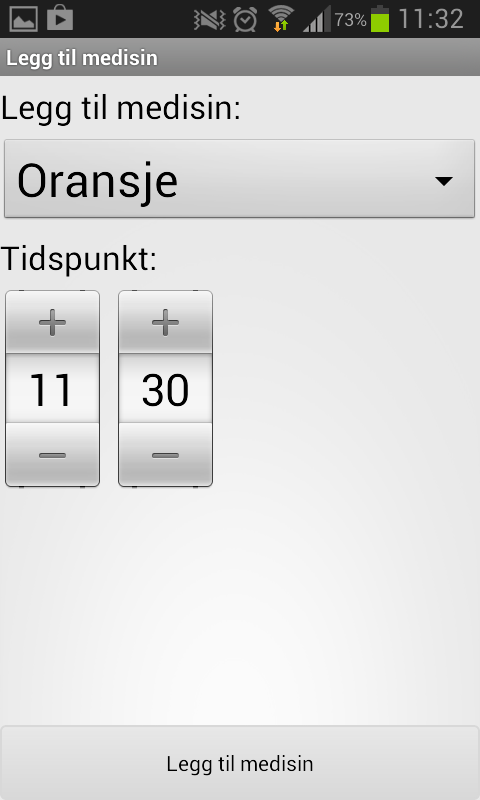
\includegraphics[width=0.20\paperwidth]{Pictures/new-screenshots/add-medicine-to-plan.png}}
		\caption{Adding a medicine to a plan}
		\label{fig:add_medicine_to_plan}
	\end{minipage}
	\hspace{3cm}
		\begin{minipage}[t]{0.4\linewidth}
		\centering
			\fbox{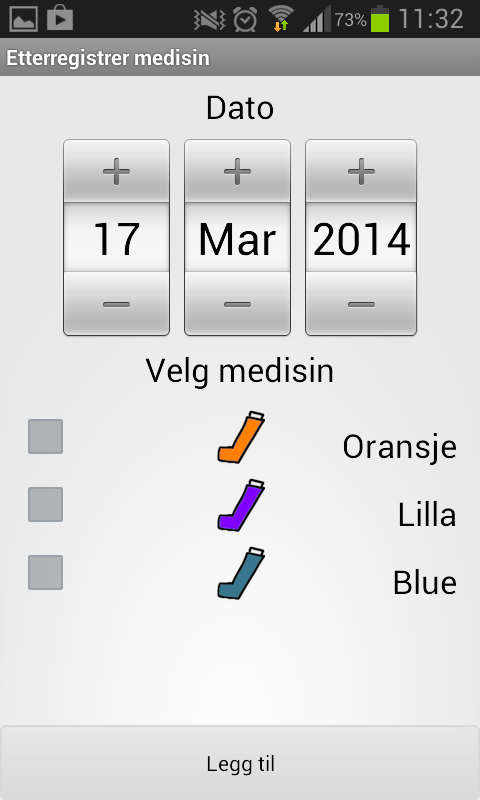
\includegraphics[width=0.20\paperwidth]{Pictures/new-screenshots/register-medicine-taken.png}}
		\caption[Register medicine taken]{Register a medicine taken}
		\label{fig:register_medicine_taken}
	\end{minipage}
	%NEW LINE
		\begin{minipage}[t]{0.4\linewidth}
		\centering
			\fbox{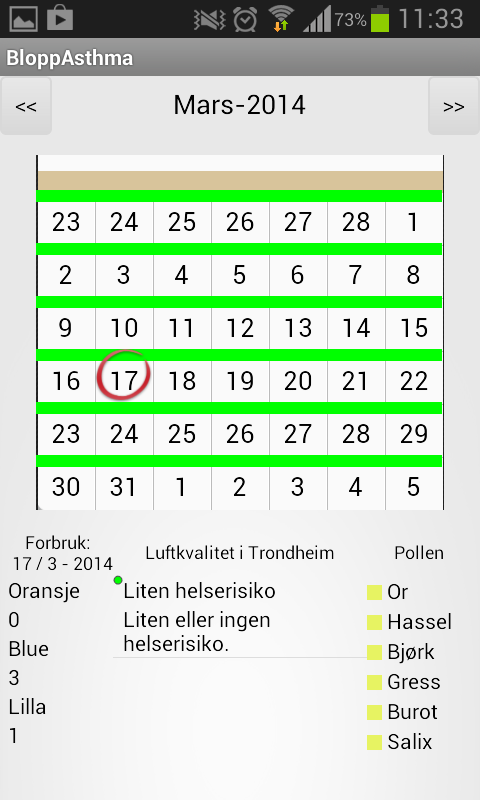
\includegraphics[width=0.20\paperwidth]{Pictures/new-screenshots/log.png}}
		\caption{Medicine log}
		\label{fig:medicine-log}
	\end{minipage}
	\hspace{3cm}
		\begin{minipage}[t]{0.4\linewidth}
		\centering
			\fbox{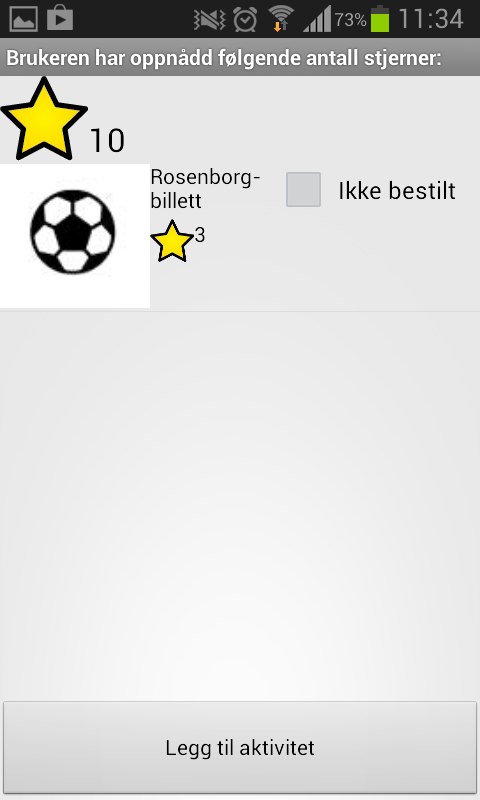
\includegraphics[width=0.20\paperwidth]{Pictures/new-screenshots/award.png}}
		\caption{Overview of rewards a child may recieve}
		\label{fig:parent-awards}
	\end{minipage}
\end{figure}

\begin{figure}
	\begin{minipage}[t]{0.4\linewidth}
		\centering
			\fbox{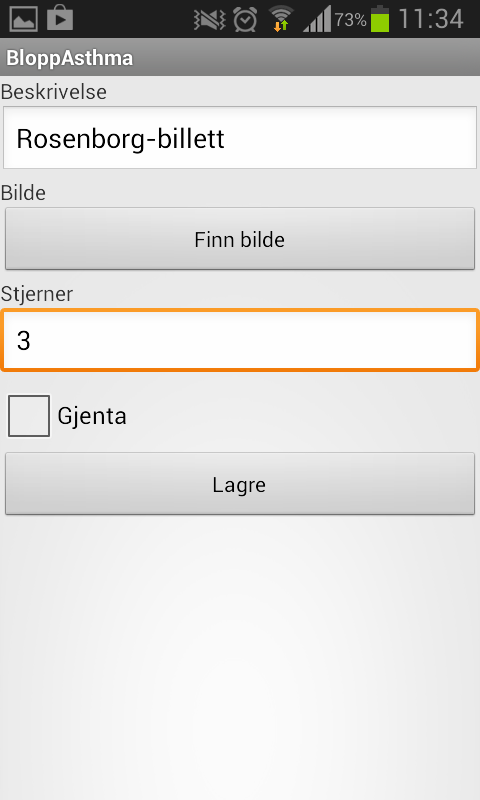
\includegraphics[width=0.20\paperwidth]{Pictures/new-screenshots/create-award.png}}
		\caption{Creating a \\ reward}
		\label{fig:parent-create-reward}
	\end{minipage}
	 \hspace{3cm}
	 \begin{minipage}[t]{0.4\linewidth}
		\centering
			\fbox{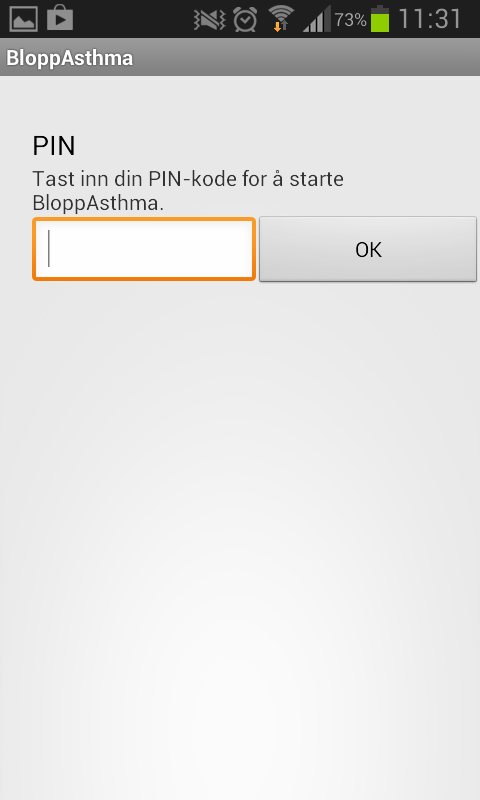
\includegraphics[width=0.20\paperwidth]{Pictures/new-screenshots/pin-challenge.png}}
		\caption{PIN challenge in parent partition}
		\label{fig:parent-pin}
	\end{minipage}
\end{figure}

\section{Parent Partition}
\label{sec:parentpartition}

A screenshot of the first view users meet is included in Figure \ref{fig:asthmapp-main-menu}. By pressing the bottom button, the user is brought to the parent partition of \app{}. 

\subsection{Menu}
\label{sec:description-menu}
Figure \ref{fig:parent_main_menu} shows the main menu of the parent partition. It has five options (Norwegian translation in paranthesis):
\begin{enumerate}
  \item Medicine Plan (\emph{Medisinplan})
  \item Register Medicine Afterwards (\emph{Etterregistrer medisin})
  \item Medicine Log (\emph{Medisinlogg})
  \item Rewards (\emph{Premier})
  \item Manual (\emph{Manual})
\end{enumerate} 

In order to access the parent partition the user is prompted with a PIN challenge. This was done in order to protect the child's medical data if a smart phone is lost or stolen. Additionally, children tampering with their medical plan or adding false treatments is avoided.

\subsection{Medicine Plan}
\label{sec:description-medicine-plan}
Creating a medicine plan for asthma treatment is highly connected to the asthma action plan explained in Appendix \ref{chp:traffic-light}.
Users can have three different plans, depending on which health state they are currently in. As we are targeting children, we cannot assume that they are aware of which category they are currently in, and as a result, we let their parents control it. Figure \ref{fig:parent_medicine_plans} and \ref{fig:add_medicine_to_plan} show the view in which one may change the medicine plan the child is currently on, in addition to setting alarms where appropriate. For instance, one may set an alarm at 07:00 AM, so it reminds the user before it is time to leave for school. Changing the medicine plan is done by selecting the checkbox at the left side of the panel.  


\subsection{Register Treatment}
\label{sec:description-register-medicine}

If a child need to take their medicine, but does not have the possibilty to do the treatment with \ab{} or \app{} nearby, they can take their medicine and register the treatment later. This ensures that children are able to collect their stars even if they did not do their treatment with \ab{} or \app{} as their companion. Figure \ref{fig:register_medicine_taken} shows how this is solved in \app{}.  

\subsection{Medicine Log}
\label{sec:description-medicine-log}
The \emph{Medicine log} can be used by parents to show how many times a child has taken his/her medicine. We assume that one of the main reasons for a child not taking his/her medicine is lack of communication between parents. A medicine log enables parents to check whether the child has taken the necessary dose on any given day.


Figure \ref{fig:medicine-log} shows the calendar view of the application, which we will explain in detail. The calendar module used is an open source component developed by Chris Goo\footnote{The source code is licensed under the Apache License, Version 2.0. At the time we wrote this thesis, we were no longer able to find the source code available online.}, which we modified for our purposes. The cells show any given day of a month. In addition, there is a top bar which shows the health state (or health plan) of the child on the day selected below. At the bottom of the screen there are three panels. The left panel shows which medicine has been taken on the selected day. The topbar of this panel indicates which day is selected. The middle panel shows the air quality in Trondheim\fnurl{Measured by NILU}{http://luftkvalitet.info/}. The right panel shows the pollen distribution of the 6 most common pollen types\fnurl{Measured by NAAF}{http://www.pollenvarslingen.no/}. The idea behind this is that asthma symptoms often correlate with allergy symptoms. If parents are able to recognize a pattern between health state and pollen distribution, they may wish to take special precautions, such as no outdoor activity on a day with extreme amounts of pollen.    


\subsection{Manual}
\label{sec:description-manual}
The manual contains the same information as shown in Section \ref{sec:description-instructions}. The manual is added to both the parent partition and the child partition of the application. This is done because it is important for both children and parents to know how to use the medicine correctly. 


\subsection{Reward}
\label{sec:description-manage-rewards}
Figure \ref{fig:parent-awards} shows the list of possible rewards a child may receive. They are added by parents through \emph{Add reward}. The idea of having parents set their children's rewards is to tailormake rewards according to children's interest (see Chapter \ref{sec:gamificationinapp}). Figure \ref{fig:parent-create-reward} shows how one may add a reward. The user inserts a description, then either adds a photo or selects one out of our standard images. It is possible to set a reward on \emph{Repeat}, which will make the reward appear multiple times, each time with an increased cost.        
When the user press \emph{Save} (Lagre), the reward is added and the child is able to select it. 
 
\section{Summary}

To build our application \app{}, we have continued development of Aaberg \etal{}'s Android applications, by focusing on a user-centered gamification system. In \app{} we have made use of three gamification mechanisms; Real-world rewards, mirroring user behavior, and experience points. 

After completing a treatment, the child is given experience points, in the shape of golden stars, based on their current health state. These stars can be used to purchase rewards defined by the child's parents. 

\app{} is an application divided into two partitions, one for parents and one for children. The parent partition give users the right to change a child's treatment plan, view a child's medicine log and add rewards that children can purchase. This partition is protected by a PIN challenge, in order to hide user data and deny children access. 

In the child partition, the child can be guided through treatments and use his/her earned stars to purchase rewards. It also gives a guide for how to perform a treatment, in the shape of a comic book.   
